\documentclass[a4paper,12pt]{article}
\usepackage[left=2.5cm,right=2.5cm,top=2.5cm,bottom=2.5cm]{geometry} 
\usepackage{color}
\usepackage[usenames,dvipsnames]{xcolor}
\usepackage{amsmath,amssymb,amsthm,algorithm,algorithmic,graphicx,yhmath,url,enumitem,lscape,mathtools}
\usepackage{wrapfig,subfigure}

\newcounter{problem}
\newenvironment{problem}{\refstepcounter{problem} \noindent {\bf Problem \arabic{problem}}}{\newpage}
\newenvironment{solution}{\vspace{0.3cm} \par \noindent {\bf Solution}}{}
\newenvironment{verification}{\vspace{0.3cm} \par \noindent {\bf Verification}}{}
\newenvironment{hint}{\vspace{0.3cm} \par {\bf Hint:}}{}

\newcounter{remark}
\newenvironment{remark}{\refstepcounter{remark} \vspace{0.3cm} \par \noindent {\bf Remark \arabic{remark}}}{\vspace{0.3cm}}
\newcounter{lesson}
\newenvironment{lesson}{\refstepcounter{lesson} \vspace{0.3cm} \par \noindent {\bf Lesson \arabic{lesson}}}{\vspace{0.3cm}}
\newcommand{\R}{\mathbb{R}}
\newcommand{\N}{\mathbb{N}}
\newcommand{\Rn}{\mathbb{R}^n}
\newcommand{\Rnn}{\mathbb{R}^{n \times n}}
\newcommand{\bes}{\begin{equation*}}
\newcommand{\ees}{\end{equation*}}
\newcommand{\be}{\begin{equation}}
\newcommand{\ee}{\end{equation}}
\newcommand{\eps}{\epsilon}
\newcommand{\fl}{\text{fl}}

\begin{document}

\title{5DV005, Fall 2018, Lab session 1}
\author{Carl Christian Kjelgaard Mikkelsen}

\maketitle
\tableofcontents

\section{The time and the place}
Our first lab session will take place on
\begin{center}
Wednesday, November 14th, 2018, (kl. 13.00-16.00), Room MA416-426.
\end{center}

\section{Compilation of \LaTeX~documents}

Documents written in \LaTeX have the extention {\tt .tex}. They are translated into .pdf files using a multi-pass compiler such at {\tt pdflatex}. The simplest case requires two pass compilation, i.e.,
\begin{verbatim}
>pdflatex lab2
>pdflatex lab2
\end{verbatim}
If the document reads a .bib file to generate a list of references, then the compilation sequence is
\begin{verbatim}
>pdflatex lab2
>bibtex lab2         
>pdflatex lab2
>pdflatex lab2
\end{verbatim}
\newpage


\section{The problems}

\begin{problem}
  \begin{enumerate}
  \item Copy the function {\tt lab2/scripts/l2p1.m} into {\tt /lab2/work/my\_sum} and identify the differences between this function and {\tt my\_simple\_sum}. In particular:
    \begin{enumerate}
    \item How is the correct value of the unit roundoff identified?
    \item What is the effect of the reshape command?
    \item How is user stupidity handled?
    \end{enumerate}
  \item Extend the function {\tt my\_sum} to include the a priori error bound given by \cite{mikkelsen2018}, Theorem 4.3. The appropriate call sequence is
\begin{verbatim}
[y, aeb, reb]=my_sum(a)
\end{verbatim}
    where
    \begin{itemize}
    \item {\tt y} is the computed sum
    \item {\tt aeb} is the a priori error bound
    \item {\tt reb} is the running error bound
    \end{itemize}
    \begin{enumerate}
    \item Remember to update the documentation.
    \item Remember to include comments related to the calculation of the error bounds.
    \item Remember to update the revision history.
    \item Remember to update the list of programmers.
    \end{enumerate}
  \item Copy {\tt scripts/sum\_mwe1.m} into {\tt work/my\_sum\_mwe1.m} and complete the script so that it computes the two sums
    \be
    a = \sum_{j=1}^n \frac{1}{j^4}, \quad b = \sum_{j=1}^n \frac{(-1)^j}{j}, \quad n = 2^{20},
    \ee
    as well as the error, an a priori error bound and a running error bound. You can obtain a \textit{very} accurate value of the true sums using Kahan's method {\tt kahan\_sum} and double precision arithmetic.
  \item Verify that the errors are bounded by the a priori error bounds.
  \item Verify that the errors are bounded by the running error bounds.
  \item Which technique gives the best error bounds?
  \item Why is it reasonable that the running error bounds are smaller than the a priori error bounds? {\bf Hint:} Which technique draws on the largest body of relevant information?
  \end{enumerate}
\end{problem}


\begin{problem}
  \begin{enumerate}
  \item Copy the incomplete function {\tt /lab2/scripts/l2p2} into {\tt /lab2/work/my\_rsum.m} and complete the function according to its specification.
  \item Extend {\tt my\_rsum} to return a running error bound.
  \item Develop a minimal working example {\tt my\_rsum\_mwe1} which computes the same sums as the previous problem using $m=2^{10}$.
  \item Verify that that the absolute value of each error is less than corresponding running error boun
  \item What are the consequences of reducing $m$ from $m=2^{10}$ to $m=1$?
    \begin{enumerate}
    \item What happens to the error?
    \item What happens to the run time? Use {\tt tic}, {\tt toc} to measure the runtime.
    \end{enumerate}
  \end{enumerate}
\end{problem}
  
\begin{problem}
  You will find the command {\tt close all} very useful for this problem.
  \begin{enumerate}
  \item Copy {\tt lab2/scripts/l2p3.m} in the function {\tt lab2/work/my\_horner.m} and complete the function according to the specification.
  \item Develop a minimal working example {\tt my\_horner\_mwe1} which plots the two polynomials
\begin{verbatim}
p = @(x)(x-2)^3
q = @(x)x.^3 - 6 x.^2 + 12 x - 8
\end{verbatim}
    for $x \in 2 + [2^{-15},2^{15}]$ using 101 equidistant points. You will allow MATLAB to compute $p$ as given, but you will apply Horner's method to evaluate $q$. Be careful and specify the coefficients in the right order!
  \item Prove mathematically that $p(x) = q(x)$ for all $x \in \R$, i.e., the two polynomials are in fact identical, although the computed values are quite different.
    \item Extend {\tt my\_horner} to include the calculation of the a priori error bound given by \cite{mikkelsen2018}, Theorem 4.10. The appropriate call sequence is
\begin{verbatim}
[y, aeb] = my_horner(a,x)
\end{verbatim}
  \item Extend {\tt my\_horner} further to include the calculation of a running error bound. The appropriate call sequence is
\begin{verbatim}
[y, aeb, reb] = my_horner(a,x)
\end{verbatim}
  \item Extend the minimal working example {\tt my\_horner\_mwe1} to create a second plot which plots the absolute value of $q$, the a priori error bound and the running error bound all in a single figure.
  \item Use the running error bound to identify the region where the sign of the computed values of $q$ can be trusted. A command such as {\tt find(a>b)} will prove useful.
  \end{enumerate}
\end{problem}

\begin{problem} In this problem you will apply the bisection algorithm to compute a firing solution for a target located at a distance $d$ from the gun. 
\begin{enumerate}
\item Read through the documentation of the function {\tt bisection} and execute the minimal working example to verify that the code makes sense. 
\end{enumerate}
In order to automatically hit a target at coordinates $(d,0)$ we have to set up a function which can be passed to the bisection algorithm along with pertinant information. The following steps takes you through this process. Rename the script {\tt lab2/script/l2p4.m} to {\tt lab2/work/l2s4.m} and completed it as suggested.
\begin{enumerate}[resume]
\item Use the minimal working example of {\tt range\_rkx.m} to initialize a gun and define a range function using those values, i.e.
\begin{verbatim}
range=@(theta)range_rkx(param,v0,theta,method,dt,maxit)
\end{verbatim}
\item Similarly, define a function which measures the distance from the point of impact to the target, i.e
\begin{verbatim}
res=@(theta)range(theta)-d
\end{verbatim} 
\end{enumerate} 
Here {\tt res} is an abbreviation of the word ``residual'', i.e. ``that which remains''. Hitting the target precisely is equivalent to solving {\tt res = 0}. In practice, we can settle for a residual which has a small absolute value, because the shell destroys anything with a certain radius $\rho$. This so-called ``kill-radius'' depends among other things on the amount and type of explosive and the type of target.

In order to use the bisection method, we need to find a bracket, i.e. a pair of angles $\theta_1$ and $\theta_2$ such that the two residuals have different signs. In terms of physics, this corresponds to firing a pair of shells such that one passes over the target and the other falls short of the target. Suitable brackets can be found if a ballistic table has already been computed.
\begin{enumerate}[resume]
\item Compute a suitable ballistic table using the function {\tt compute\_range}.
\item Explain to your friends, why the command {\tt find(table(2,:)>d)} can be used to rapidly determine a bracket!
\item Compute the elevation necessary to hit a target at $d = 12345$ using the bisection algorithm. Xenomorphs are very sturdy, so we want a residual which is less than 1 meter. Moreover, we want both the high and the low angle. Use the function {\tt range\_rkx} to generate the trajectories and plot them in the same figure. You should end up with a figure which looks like Figure \ref{trajectories}.

\begin{figure}
\centering
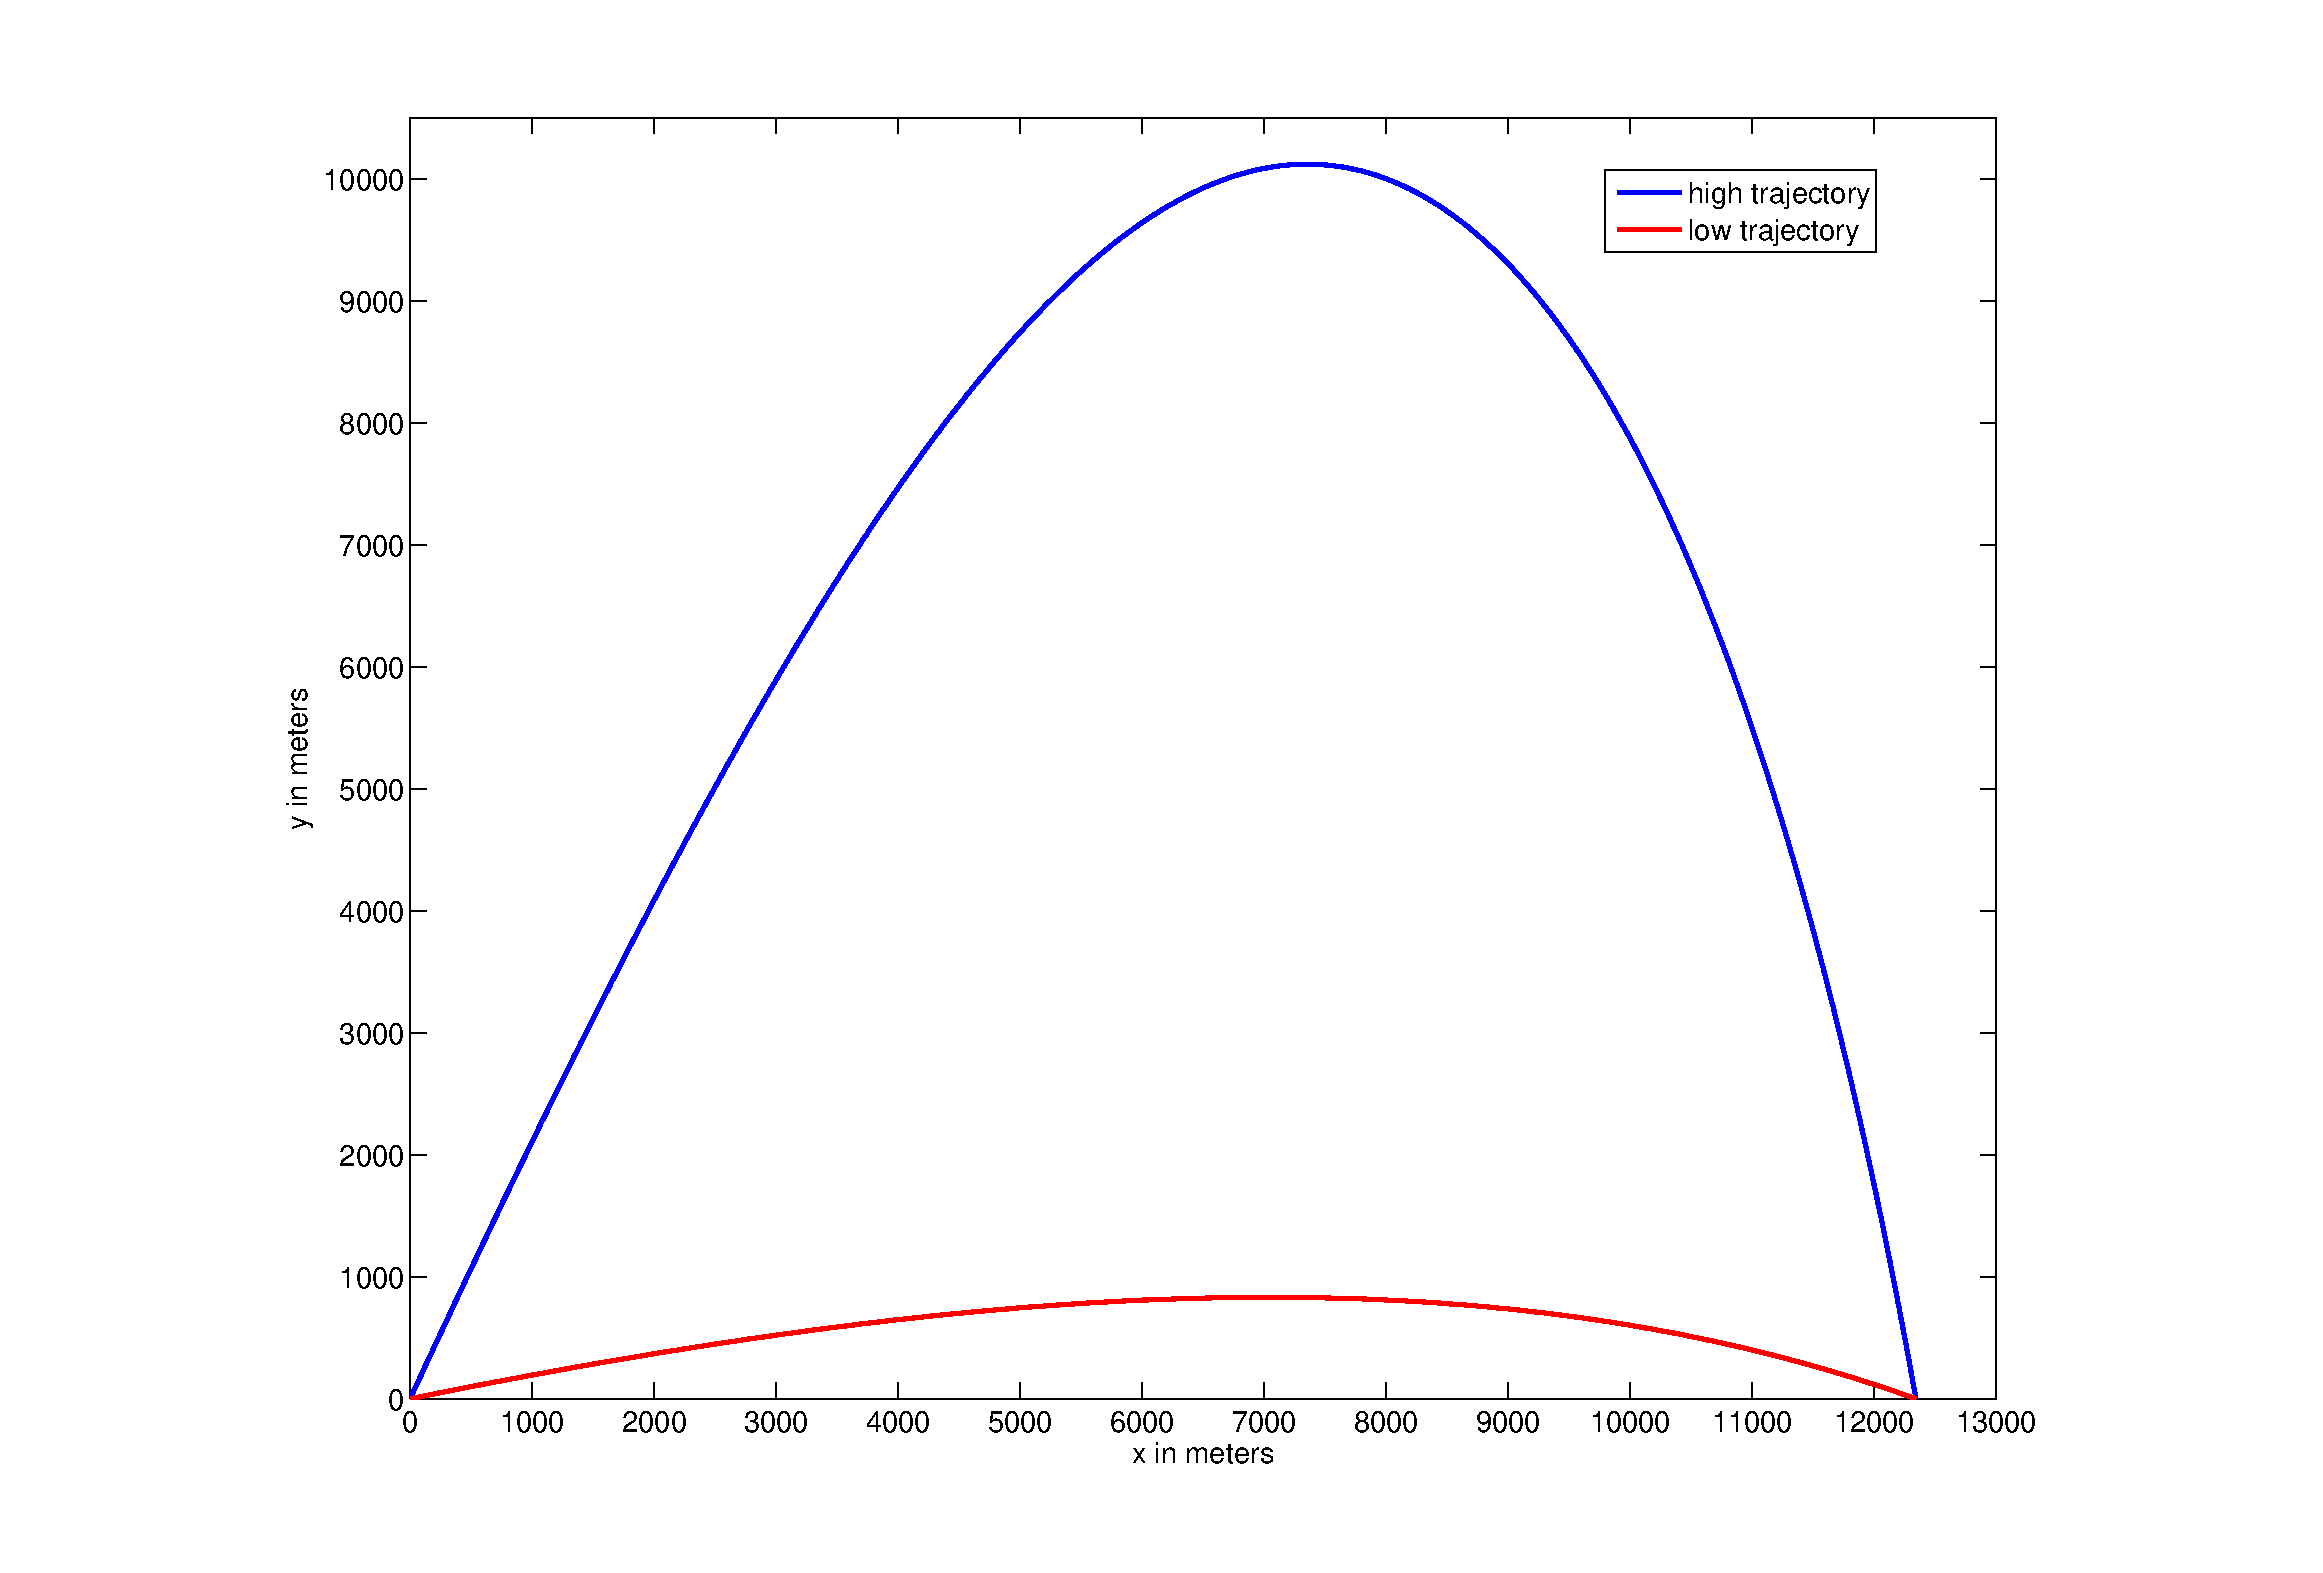
\includegraphics[width=14cm]{trajectories.pdf} \caption{A plot of the high and the low trajectories for hitting a target at {\tt d = 12345}.} \label{trajectories}
\end{figure}

\item A UAV (Unmanned Aerial Vehicle, i.e. a drone) has spotted a group of xenomorphs hiding behind a large hill. Your friend has analyzed the telemetry and gives you the new range. Compute the high and the low trajectory. Explain why the high trajectory is the probably the only viable option.
\end{enumerate}
\end{problem}

\section{Concluding remarks}

\begin{enumerate}

\item Programs without proper description of the call sequence, input/output specification are useless to the user and the next programmer. Programs without meaningful comments are impossible to maintain. Good programmers are not afraid of writing their name on their products. Without contact information it is impossible to report bugs or ask for clarification.
  \begin{center}
    {\bf Programs which do not follow these principles will not be accepted.}
  \end{center}

\item Recursion is an elegant solution to many problems, but be wary of the overhead incurred by the function calls. Recursion is appropriate when the overhead is insignificant compared with the actual computation. This is not case if the computation consists of a single addition. Your recursive summation function uses a threshold {\tt m} which sacrifies some accuracy for the sake of speed. It is possible to do tree-wise summation without recursion, but the code is a tad more complicated as demonstrated by {\tt tree\_sum}.

\item There is a lesson to be learned from question about the UAV. You should never blindly rely on the numbers generated by a computer. Always ask yourself what the numbers mean in the real world. In this case the low trajectory is likely to intersect the hill and it is useless for the practical purpose of destroying the xenomorphs. The hill is not part of the simulation, but it is part of the real world. The low trajectory is a valid firing solution, but only within the confines of the simulation.

\end{enumerate}

\bibliographystyle{plain}
  \bibliography{../../../lecture-notes/refs}
  
\end{document}





